\SACCMD{map}
\label{cmd:map}

\SACTitle{概要}
利用SAC内存中的所有数据文件生成一个包含台站/事件符号、地形以及台站名的
GMT地图,也可以在命令行上指定一个事件文件。每个地震事件符号可以根据震级、
残差等确定其大小。这个命令会产生一个PS文件,并将该文件在屏幕上显示,同时
产生一个绘制该图的shell脚本。

\SACTitle{语法}
\begin{SACSTX}
MAP [MER!CATOR!|EQ!UIDISTANT!|AZ!IMUTHAL_EQUIDISTANT!|ROB!INSON!]
    [WEST minlon] [EAST maxlon] [NORTH maxlat] [SOUTH minlat]
    [MAG!NITUDE!|RE!SIDUAL!|RM!EAN_RESIDUAL!] [EV!EVNTFILE! filename]
    [TOPO!GRAPHY!] [STAN!AMES!] [MAPSCALE on|off] [PLOTSTATIONS on|off]
    [PLOTEVENTS on|off] [PLOTLEGEND on|off] [LEGENDXY x y]
    [FILE output-file]
\end{SACSTX}

\SACTitle{输入}
SAC中可以使用的投影方式包括:
\begin{itemize}
\item \texttt{MERCATOR}:投影方式为Mercator投影
\item \texttt{EQUIDISTANT}:投影方式为等间距圆柱投影,经纬度为线性
\item \texttt{ROBINSON}:投影方式为Robinson投影,适用于世界地图
\item \texttt{LAMBERT}:适用于东西范围较大的区域
\item \texttt{UTM}:通用横向Mercator(尚未实现)
\end{itemize}

下面的选项允许用户指定地图的区域,其默认使用台站以及事件经纬度的最小
最大值(如果真是如此,这样的缺省值并不合适,因为那样意味着某些台站或事件
将位于地图的边界处,但是实际上地图范围给的还是不错的):
\begin{itemize}
\item \texttt{WEST}:地图的最小经度
\item \texttt{EAST}:地图的最大经度
\item \texttt{NORTH}:地图的最大纬度
\item \texttt{SOUTH}:地图的最小纬度
\item \texttt{AUTOLIMITS}:自动决定地图的区域 [缺省值]
\end{itemize}

下面的选项允许用户向地图中添加位置和注释:
\begin{itemize}
\item \texttt{STANames on|off}:在地图上绘制台站名[默认为off]
\item \texttt{MAPSCALE on|off}:在地图上绘制地图比例尺[默认为off]
\item \texttt{PLOTSTATIONS on|off}:绘制地震图给出的全部台站[默认为on]
\item \texttt{PLOTEVENTS on|off}:绘制eventfile和/或地震图给出的全部事件
    [默认为on]
\end{itemize}

下面的选项允许用户根据不同的值给出不同地震事件符号的大小。默认值是所有
符号大小一样:
\begin{itemize}
\item \texttt{MAGnitude}:\texttt{user0} 定义地震震级,\texttt{user0} 越大,
    则事件符号越大
\item \texttt{REsidual}:\texttt{user0} 定义残差。根据 \texttt{user0} 的
    绝对值定义事件符号的大小。正值为\texttt{+} 负值为 \texttt{-}
\item \verb|RMean_residual|:与residual相同,除了将所有残差去除均值之外
\item \texttt{PLTLEGEND on|off}:绘制地震震级以及残差的图例[默认为on]
\item \texttt{LEGENDXY x y}:绘制图例的绝对位置,默认为 \texttt{[1,1]}。
    位置是相对于页面的左下角,其单位为inch。这是一个与地震震级和残差有关
    的图例。
\item \texttt{EVENTFILE}:指定一个自由格式的ASCII文本文件,其包含了额外的
    事件数据,文件的每一行包含单个事件的数据。每行的头两列必须包含纬度和
    经度(单位为度)。第三列可以包含符号大小信息(比如震级、深度、走时残差等)。
\item \texttt{TOPOgraphy on|off}:设置TOPO为开允许用户向地图中添加地形和
    海洋深度。该命令读取GMT中 \texttt{grdraster.info} 的第一个地形文件,
    当然地形文件中必须要有该区域的数据。地形彩色图使用
    \verb|$SACAUX/ctables/gmt.cpt|。网格文件被写入当前目录
\item \texttt{FILE}:默认的输出文件名为 \texttt{gmt.ps},你可以通过
    \texttt{FILE} 选项指定文件名
\end{itemize}
可以用SAC的 \nameref{cmd:title} 命令指定地图标题。

\SACTitle{缺省值}
\begin{SACDFT}
map mercator topo off stan off file gmt.ps plotstations on
    plotevents on
\end{SACDFT}

\SACTitle{示例}
利用SAC提供的一些数据作为例子:
\begin{SACCode}
SAC> dg sub regional *.z
SAC> title "Station Location Map"
SAC> map stan on
Using Default Postscript Viewer
	gs -sDEVICE=x11 -q -dNOPROMPT -dTTYPAUSE
\end{SACCode}
绘制出的地图如图 \ref{fig:map} 所示,整个地图的边界控制的还算不错,还算
比较美观,三角形代表台站位置,圆形代表地震位置,大小也控制的不错。生成这
个图的同时,还有一个可以用于生成该地图的shell脚本。

默认情况下,该命令会自动使用gs预览生成的PS文件。如果想用其他PS阅读器预览,
可以通过修改环境变量 \texttt{SACPSVIEWER} 来实现,比如
\texttt{export SACPSVIERER=evince}。

\begin{figure}[!ht]
\centering
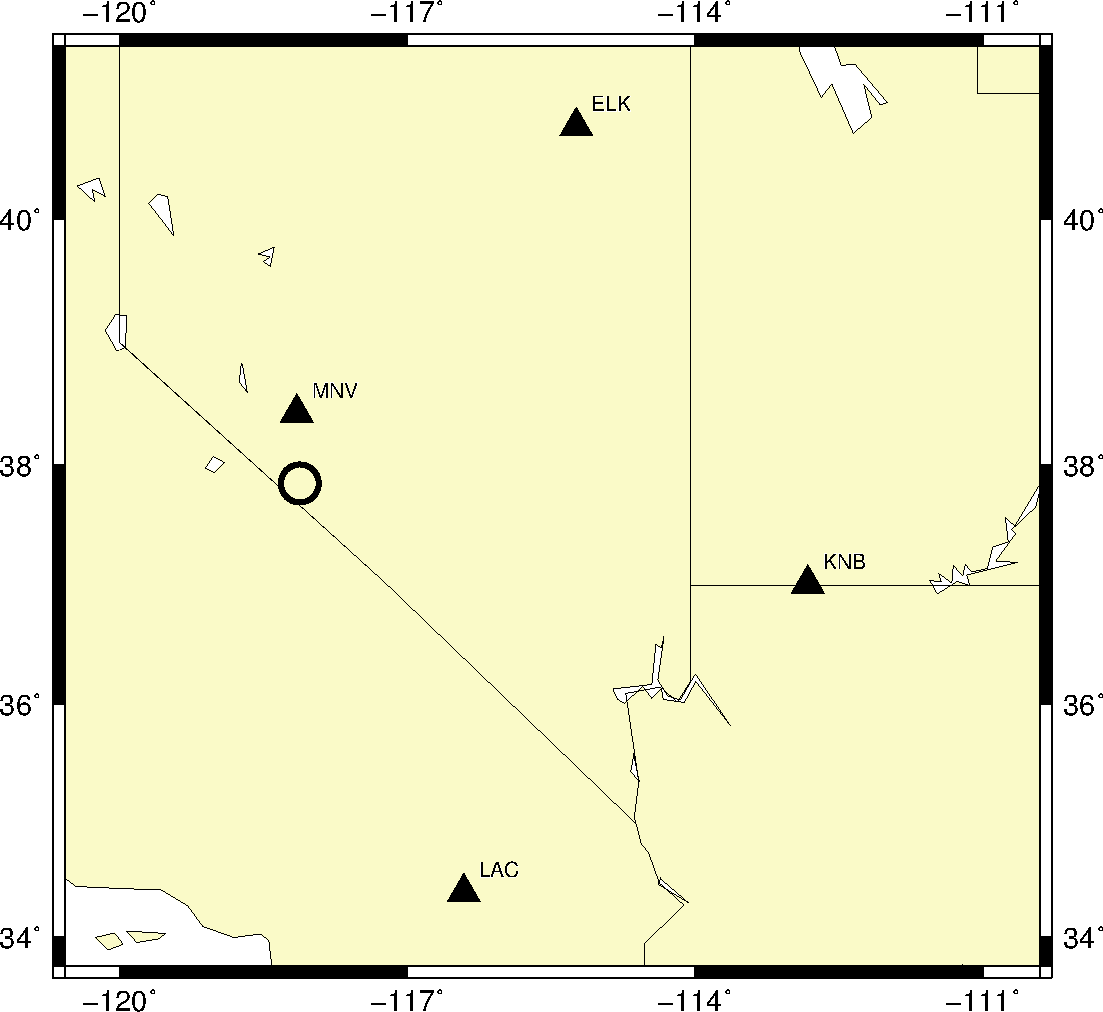
\includegraphics[width=0.7\textwidth]{map}
\caption{map绘制地震、台站分布图}
\label{fig:map}
\end{figure}

\SACTitle{头段数据}
台站纬度(\texttt{stla})以及经度(\texttt{stlo})必须在头段中被定义。
如果事件纬度(\texttt{evla})以及经度(\texttt{evlo})被定义则其会被包含
在地图中。如果这个命令在执行 \nameref{cmd:bbfk} 之后执行,\texttt{map}
将沿着反方位角方向绘制大圆弧路径。这个版本的 \texttt{map} 是基于4.0版本的
Generic Mapping Tools,要执行这个命令,你需要将GMT4.0安装在你的机器上并
保证可执行文件位于路径中。

每个 \texttt{map} 命令的结果将写入当前目录下一个称为 \texttt{gmt.csh} 的
脚本中。用户可以修改这个文件以利用更多SAC未利用的选项。默认单位是inch,
当然可以在脚本中修改。

在使用 \texttt{pscoast} 绘制海岸线时,SAC采用了 \texttt{-Dl} 选项,其中
\texttt{l} 代表低精度的海岸线数据。用户可以在脚本中修改使用更高精度的
海岸线数据。
